%%%%%%%%%%%%%%%%%%%%%%%%%%%%%%%%%%%%%%%%%%%%%%%%%%%%%%%%%%%%%%%%%%%%%%%%%%%%%%%%
% IEEE short-paper source aligned to the professor-edited PDF supplied 2026-08-06.
% Scientific content and reported values are limited to that supplied document.
\documentclass[letterpaper,10pt,conference]{ieeeconf}

\IEEEoverridecommandlockouts
\overrideIEEEmargins

\usepackage{amsmath}
\usepackage{array}
\usepackage{booktabs}
\usepackage{cite}
\usepackage{graphicx}
\usepackage[bookmarks=false,colorlinks=true,linkcolor=black,citecolor=black,urlcolor=blue]{hyperref}

\newcommand{\doi}[1]{\href{https://doi.org/#1}{doi: #1}}

\ifdefined\anonymoussubmission
\hypersetup{
  pdftitle={CATEM: A Timestamp-Aware Cross-Layer Framework for Telepresence Evaluation},
  pdfauthor={Anonymous},
  pdfsubject={IEEE short-paper review manuscript},
  pdfkeywords={telepresence, measurement framework, evidence traceability}
}
\else
\hypersetup{
  pdftitle={CATEM: A Timestamp-Aware Cross-Layer Framework for Telepresence Evaluation},
  pdfauthor={Sara Falcone and Teja Maheshwara},
  pdfsubject={IEEE short paper},
  pdfkeywords={telepresence, measurement framework, evidence traceability}
}
\fi

\title{\LARGE \bf
CATEM: A Timestamp-Aware Cross-Layer Framework for Telepresence Evaluation
}

\ifdefined\anonymoussubmission
\author{\mbox{}}
\else
\author{\mbox{}}
\fi

\begin{document}

\maketitle
\thispagestyle{empty}
\pagestyle{empty}

\begin{abstract}
In telepresence research, experiments often integrate subjective surveys, behavioral monitoring, physiological data collection, robot telemetry, and network analysis. Despite these sources addressing the same task, they are usually gathered separately, complicating the examination of how diverse evidence connects to a common event or the replication of the logic behind reported outcomes. Current tools assess individual constructs, synchronization techniques align the data, and dashboards display the findings. However, our literature review did not reveal a telepresence-specific measurement contract (a standardized framework for record structure, semantics, and evidence traceability) bridging data collection and interpretation. We introduce CATEM, a telepresence-specific measurement and reporting framework built around this contract. It preserves each record's construct identity, provenance, missingness, and transformation history. Interpretation limits remain explicit as diverse evidence is linked to shared task events. CATEM intentionally avoids creating a universal telepresence score. It separates evidence across experience, action, human state and cognition, and system observations, along with overarching Data and Interpretation Conditions. An executable reference implementation facilitates stored sessions, live telemetry, event-focused analysis, and traceable exports. Software verification demonstrates conformance to the specified contract and transparent handling of controlled faults. These findings support implementation behavior rather than construct validity, predictive performance, researcher utility, or causal links.
\end{abstract}

\noindent\textit{Keywords} - Telepresence evaluation, measurement framework, evidence traceability, multimodal synchronization, reproducibility.

\begingroup
\renewcommand\thefootnote{}
\footnotetext{Source code, sample data, the event fixture, and verification artifacts are available at \url{https://github.com/tejamah/telepresence_metrics_dashboard/tree/v0.2.0}.}
\addtocounter{footnote}{-1}
\endgroup

\section{INTRODUCTION AND MOTIVATION}

Telepresence systems integrate immersive displays, remote robotics, tracking, haptics, shared autonomy, physiological sensing, and networked controls. Their assessment is diverse: presence and agency capture the experience; time and error reflect actions; workload and physiology indicate human state and cognition; while latency, packet loss, and tracking detail the technical pathway. These metrics complement each other and are not interchangeable \cite{kilteni2012,hart1988,steinfeld2006}.

However, research often logs each data source separately. Imagine an operator remotely managing a robot that drops an item. Analyzing this incident might involve reviewing robot and network logs, workload metrics, physiological and tracking data, and survey responses. Different clocks and sampling rates can obscure changes occurring before, during, and after the drop \cite{falcone2024calibration}. Neither average scores nor separate dashboards address the issue of temporal evidence.

Why choose CATEM over a standard multimodal pipeline? Data-fusion methods focus on how to combine signals, and dashboards on how to present results. CATEM instead organizes and presents diverse measurement evidence that must remain intact from collection to interpretation; it does not introduce new telepresence metrics or replace validated tools. Its integration unit is a traceable measurement record, not a fused feature vector or a composite telepresence score. The record retains the meaning of each construct while making provenance, missing data, transformations, clock quality, and interpretation limits visible across sources.

This paper offers four contributions: (1) a telepresence-specific measurement contract that maintains construct identity, units, provenance, missing data, transformations, and interpretation boundaries; (2) a distinct cross-cutting condition set that supports, but is not part of, the four observational layers; (3) non-causal event-centered synchronization across diverse records; and (4) an open executable reference implementation supporting stored sessions, live telemetry, a versioned event-window endpoint, and traceable exports.

\section{RELATED WORK}

Existing research provides important foundations for the individual aspects of telepresence evaluation. Presence and embodiment research distinguishes mediated location, ownership, agency, and self-location \cite{slater1997,kilteni2012}. Falcone \emph{et al.} provided a review and practical toolbox for designing and assessing embodiment in teleoperation \cite{falcone2023}; their subsequent empirical work related embodiment to motor learning and adaptation while retaining task and system context \cite{falcone2024}. Workload instruments and physiological sensing characterize task demands and operator responses \cite{hart1988,meehan2002}, whereas human--robot interaction evaluation includes performance, autonomy, safety, trust, and physical interaction experience \cite{steinfeld2006,goodrich2008,seifi2024}. Teleoperation research separately emphasizes delay and control stability \cite{hokayem2006}. Contemporary immersive systems also compare visual conditions and spatial representations for robot control \cite{gloumeau2024}. Multisensor and multimodal research provides general methods for combining temporally related signals \cite{hall1997,baltrusaitis2019}.

Existing approaches typically address part of the evaluation problem: validated instruments measure individual constructs, middleware records technical telemetry, multimodal methods align or fuse signals, and dashboards visualize outputs. Adjacent standards address neighboring problems. LSL synchronizes independently clocked streams on a common timebase through per-sample timestamps and clock correction \cite{kothe2025}; BIDS organizes and describes the outputs of a domain's experiments through a community file and metadata structure \cite{gorgolewski2016}; FAIR states general principles for findable, accessible, interoperable, and reusable data \cite{wilkinson2016}; and PROV-O provides a general vocabulary for representing provenance \cite{lebo2013}. None is telepresence-specific, and none binds construct identity, expected-but-absent measures, and interpretation boundaries to the runtime path from ingestion through alignment to export. CATEM can use these mechanisms, but its claim is different: it defines an executable interface contract across the evidence lifecycle. The contract imposes testable invariants---properties that must remain true through ingestion, alignment, display, and export. Construct and unit identity remain attached to records, expected-but-absent measures remain explicit, transformations and provenance remain traceable, event alignment remains inspectable, and $\mathcal{D}_{t}$ remains a qualifier rather than an outcome layer. CATEM's novelty therefore lies not in a new metadata field or synchronization algorithm, but in this telepresence-specific combination and preservation boundary between instrumentation and analysis. Based on the reviewed literature, we did not identify a telepresence-specific contract serving this role. CATEM complements schemas, ontologies, instruments, middleware, synchronization methods, and statistical models; it does not replace them.

\section{CATEM FRAMEWORK}

\subsection{Design Principles}

CATEM follows three design principles: construct preservation, evidence traceability, and event-centered synchronization. \emph{Construct preservation} keeps experiential, behavioral, physiological, and technical measures distinct, preventing a favorable value in one domain from substituting for evidence in another. \emph{Evidence traceability} retains raw values, units, source metadata, missingness, registered transformations, and interpretation boundaries so that a researcher can reconstruct how a display or prototype summary was produced. \emph{Event-centered synchronization} aligns records around task-relevant events while retaining the original sampling context. It supports the inspection of what changed together without interpreting temporal proximity as a causal effect.

A measurement contract standardizes record structure and semantics for representation, synchronization, traceability, and interpretation; it does not prescribe metric computation or validation. Unlike a schema or ontology alone, the contract couples those semantics to preservation requirements that the implementation can test across processing stages. CATEM is neither a psychometric instrument, universal score, nor an automated diagnosis of teleoperation failures.

\subsection{Layered Evidence Model}

For a session window $t$, CATEM represents the evidence profile as
\begin{equation}
\mathbf{L}_{t}=[L_{E,t},L_{A,t},L_{H,t},L_{S,t}],
\label{eq:layers}
\end{equation}
where $E$ is experience, $A$ is action, $H$ is human state and cognition, and $S$ is system conditions. A separate set, $\mathcal{D}_{t}$, contains clock quality, missingness, provenance, transformation history, reliability evidence, and interpretation boundaries. Here, \emph{clock quality} denotes the estimated timestamp-alignment error, in milliseconds, relative to the study's reference time base; a deployment may additionally report clock offset, drift, and correction method. The auditable evidence view is $\mathcal{E}_{t}=(\mathbf{L}_{t},\mathcal{D}_{t})$; $\mathcal{D}_{t}$ qualifies records across the four layers but does not constitute a fifth layer. Equation~(\ref{eq:layers}) provides an organizational perspective rather than a latent ``telepresence'' construct or causal graph. Without temporal alignment, it is impossible to interpret relationships between operator behavior, system performance, and subjective experience within the same event context.

Expected but absent fields remain as explicit null records. For expected set $E_{\ell}$ and observed set $M_{\ell}$, layer coverage is
\begin{equation}
C_{\ell}=\frac{|M_{\ell}|}{|E_{\ell}|}.
\label{eq:coverage}
\end{equation}
Synchronization quality, missing-data burden, provenance completeness, and available reliability evidence are reported separately from prototype layer summaries. In practice, a missing sensor changes the evidence condition instead of being silently treated as a poor outcome for humans or systems.

The metrics remain separate. Optional prototype layer summaries are calculated from registered, normalized within-layer transformations. Prototype layer summaries use fixed equal weights solely to verify software behavior; they are not validated scales, empirical scores, or recommended aggregation methods. These summaries are optional navigation aids; CATEM's core synchronized and traceable evidence representation does not require aggregation. Reports retain the original observations and do not require a universal score. Every registered transformation emits its inputs and a readable evidence trace. This supports comparison and hypothesis generation while keeping analytic choices visible; temporal co-occurrence alone does not imply causality.

CATEM is not intended to replace validated questionnaires, robot middleware, synchronization libraries, statistical analysis packages, or predictive models. It provides a standardized evidence layer through which outputs from these existing tools can be interpreted together.

\subsection{Measurement Contract}

Each measurement entry maintains its metric and construct identifiers, layer, unprocessed value, unit, timestamp, sensor or instrument, sampling frequency, valid range, preprocessing details, origin, transformation version, and interpretation boundary.

Typically, a researcher accesses the standard object-drop window, examines a common time frame across the four observational layers, and traces any displayed value back to its measurement entries. In the object-drop scenario, this process addresses inquiries such as whether network degradation, tracking loss, increased workload, and diminished agency were documented within the same time frame, whether any anticipated stream was missing, and whether a transformation or clock-quality alert influenced interpretation. CATEM does not determine which factor led to the drop. It organizes the shared-time evidence necessary to develop testable hypotheses and decide on the need for additional instrumentation or controlled comparisons.

\section{PROTOTYPE ARCHITECTURE}

The prototype processes stored sessions, real-time telemetry, and a standard event fixture through the views shown in Fig.~\ref{fig:dashboard}. Its measurement contract ensures the retention of fields necessary for alignment and traceability before the CATEM engine generates layer views and related Data and Interpretation Conditions. React offers an interface for researchers, while FastAPI handles sessions in comma-separated-value (CSV) format and live WebSocket telemetry and manages event-window requests. Rule evaluation results in traces that can be inspected. The dashboard presents results from the JavaScript Object Notation (JSON) API, and the verification harness outputs JSON and CSV artifacts. The recommendations shown are for informational purposes; the prototype neither operates a robot nor autonomously modifies an interface.

\begin{figure*}[t]
\centering
\begin{minipage}{.96\textwidth}
  \centering
  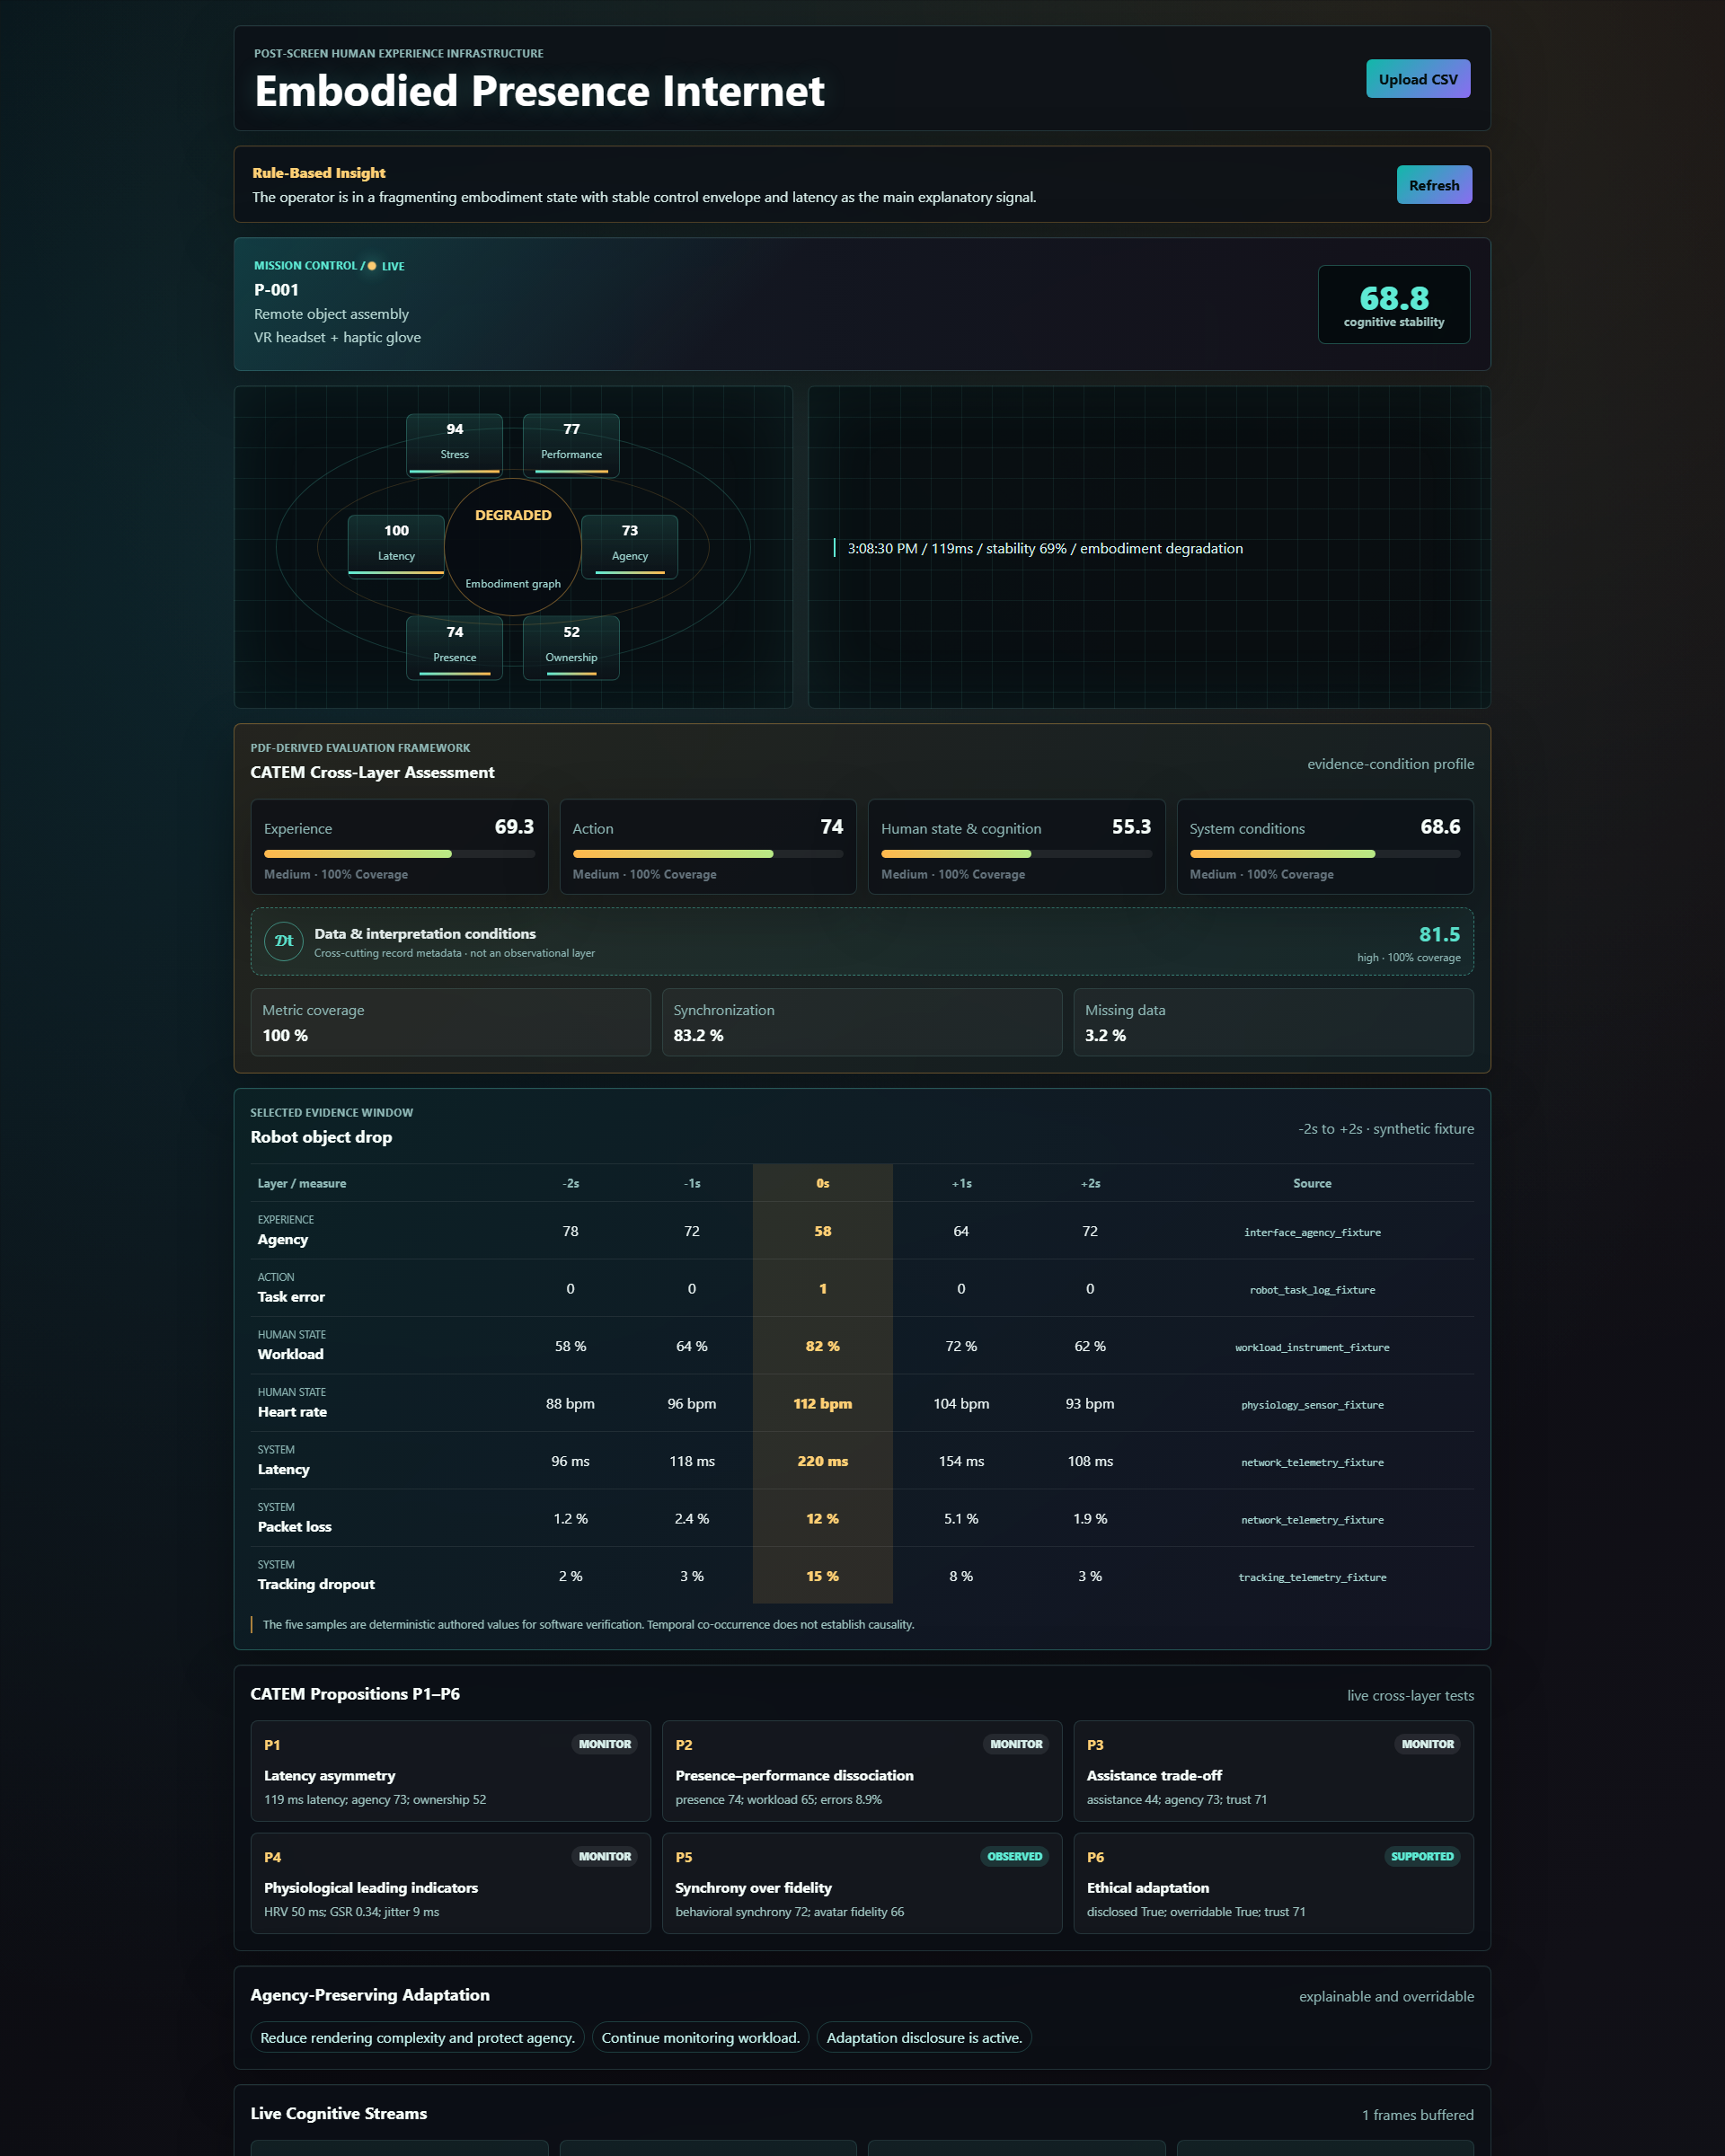
\includegraphics[width=\linewidth,trim=260bp 1200bp 260bp 790bp,clip]{figures/dashboard_overview_full.png}\\[-0.5mm]
  {\footnotesize (a) Four observational layers and the separate $\mathcal{D}_{t}$ condition band}
\end{minipage}\\[2mm]
\begin{minipage}{.96\textwidth}
  \centering
  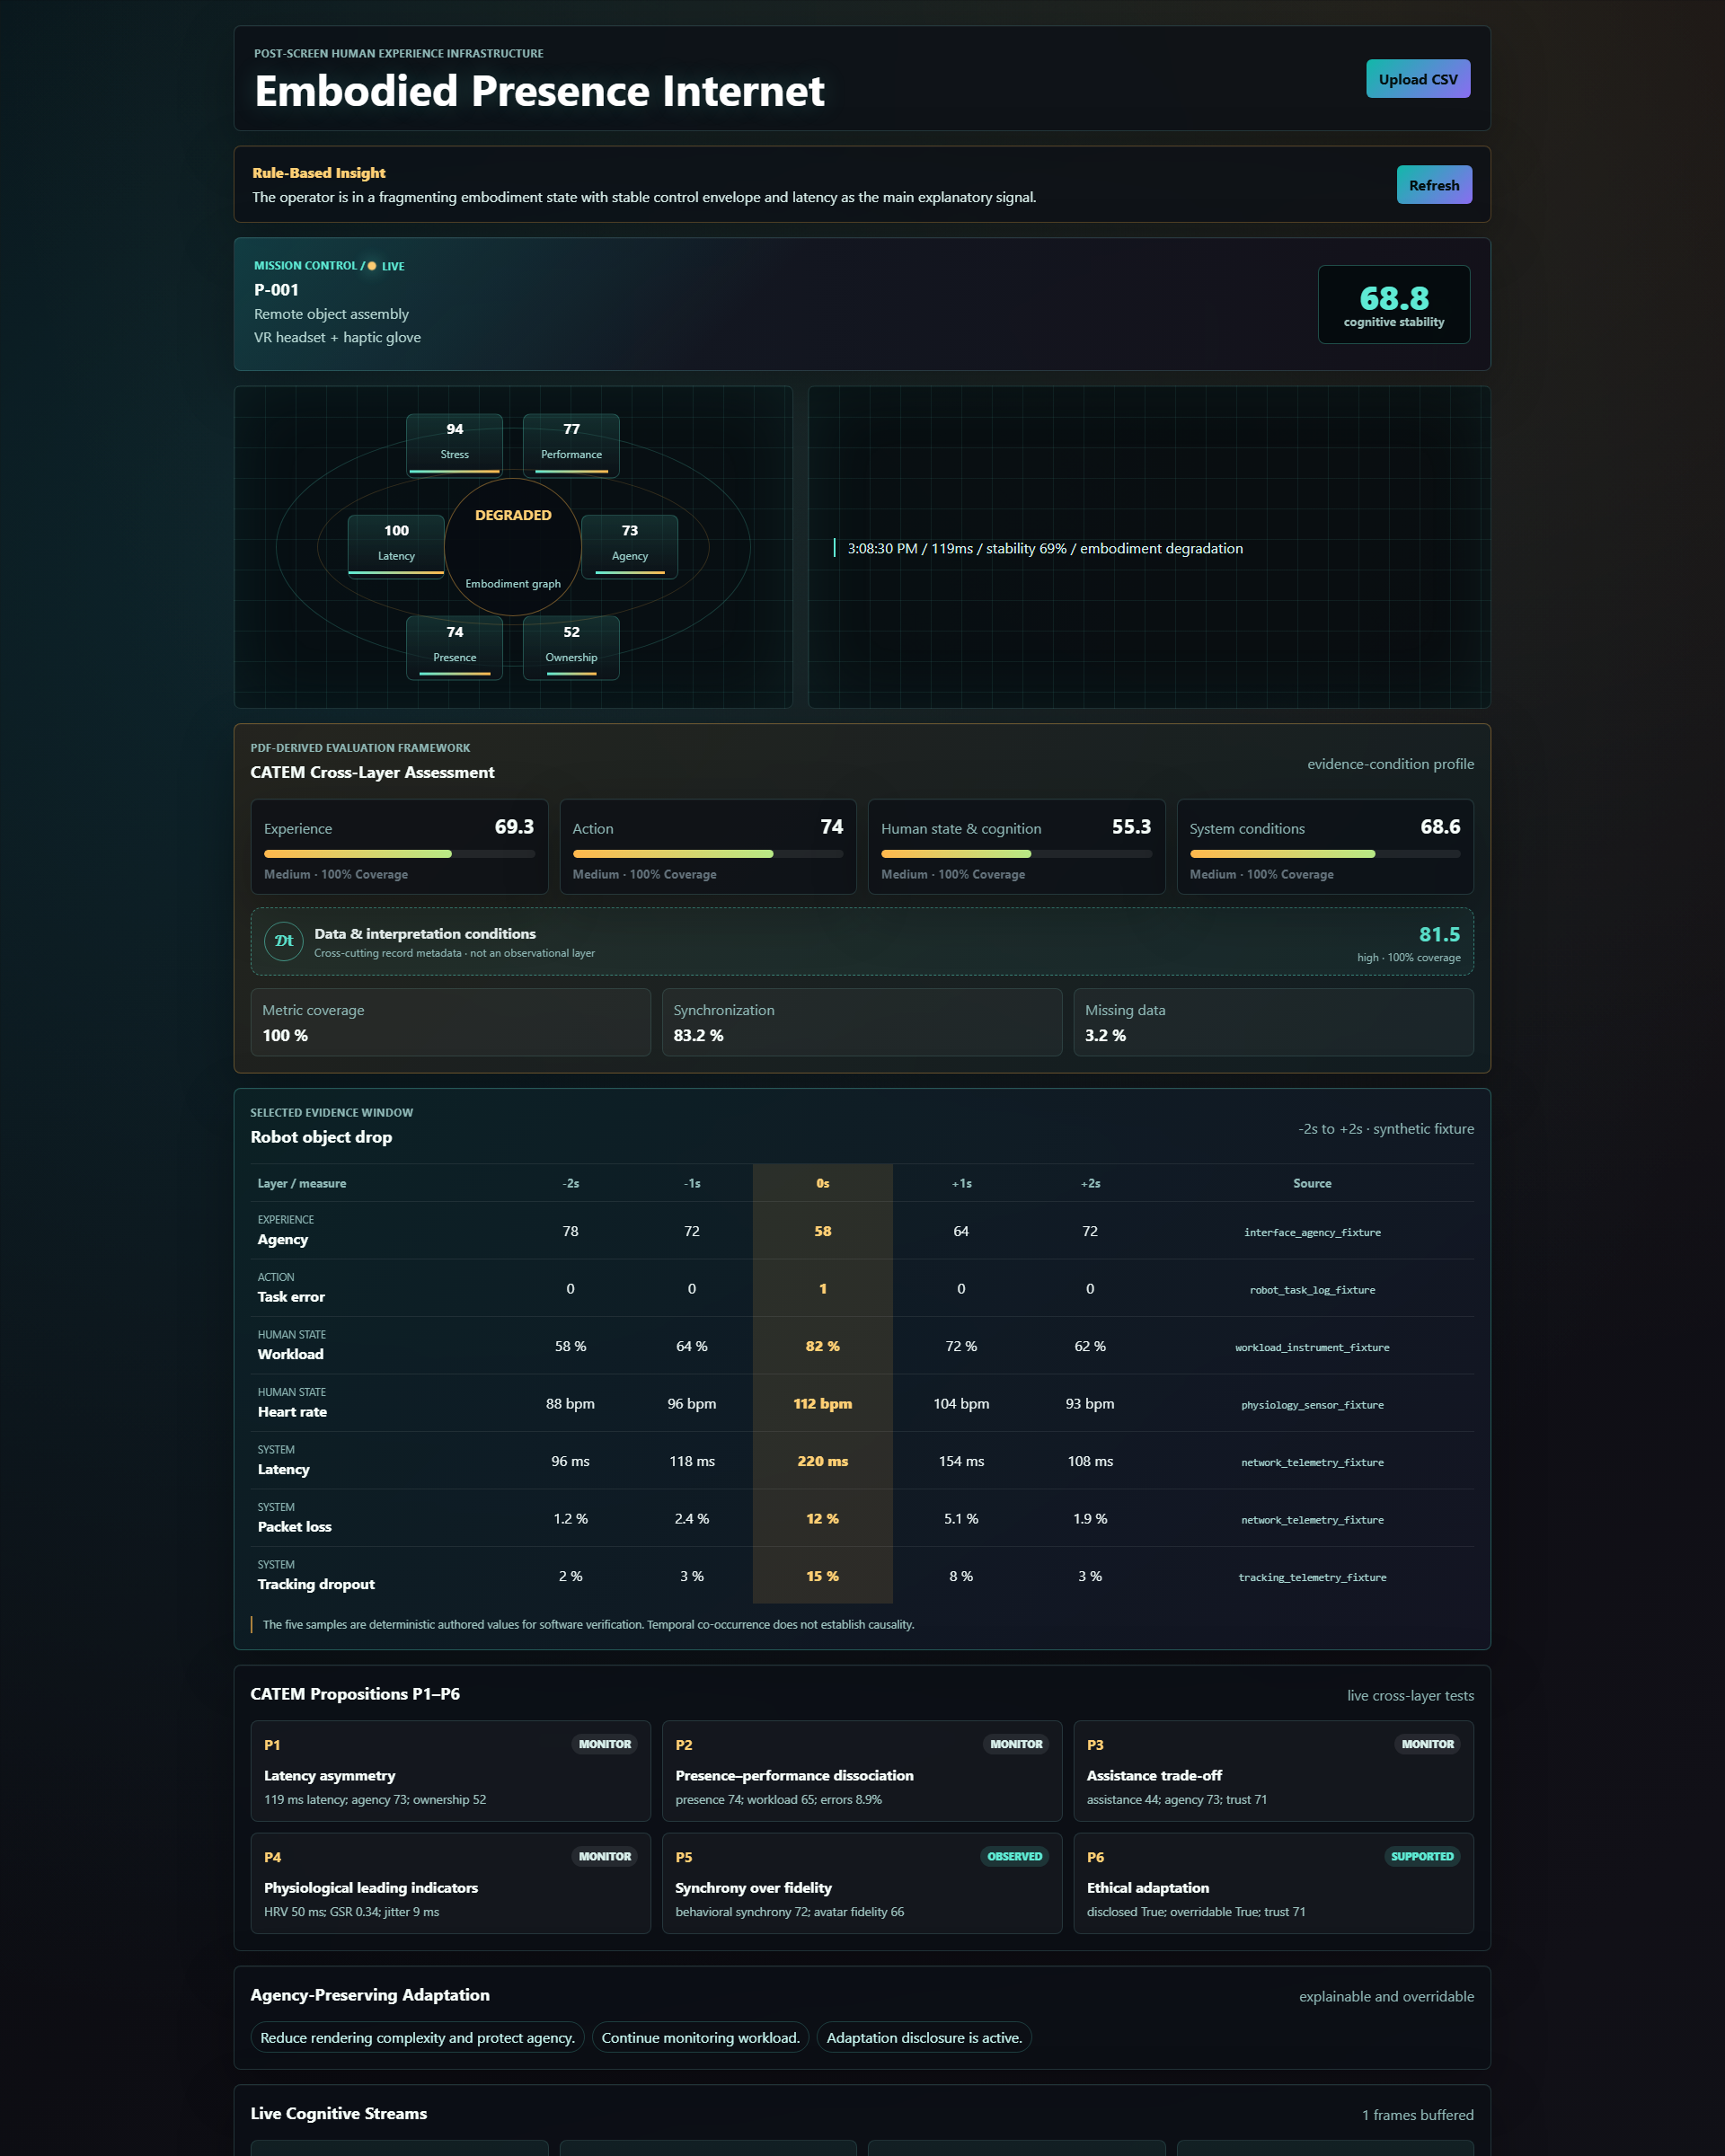
\includegraphics[width=\linewidth,trim=260bp 550bp 260bp 1180bp,clip]{figures/dashboard_overview_full.png}\\[-0.5mm]
  {\footnotesize (b) Synthetic object-drop evidence window}
\end{minipage}
\caption{Implemented CATEM dashboard views. Panel (a) keeps Data and Interpretation Conditions separate from the four observational layers; panel (b) shows seven measures at five timestamp offsets with their record sources. All values are authored synthetic demonstration data used solely for software verification.}
\label{fig:dashboard}
\end{figure*}

\section{SYNTHETIC CASE STUDY}

\subsection{Scenario and Fixture Design}

We employed software verification because the main focus of this study is conformance to and transparency of the measurement contract, rather than human effectiveness or construct validity. The tests evaluate whether CATEM can process diverse measurements, align them using timestamp offsets, maintain layer distinctions, identify missing data, react directionally to known faults, and produce inspectable evidence for researcher interpretation.

Two authored session summaries test stored-session processing. Session~1 depicts remote assembly with moderate workload, effective tracking, and successful manipulation. Session~2 illustrates a degraded remote-navigation summary with increased tracking dropout, workload, task error, and reduced agency. Its stored latency and packet-loss values were lower than those in Session~1 and were not used to assert network degradation.

A separate event fixture depicts an operator transferring an object, with the remote robot dropping it at $t=0$. CATEM aligns the robot, network, tracking, interface, workload, and physiological records around the marker. Synthetic values were chosen as deterministic fixtures covering nominal and degraded operating conditions. They were not sampled from participants and were not intended as population thresholds. We defined the expected directional responses before replay and used them solely to verify implementation behavior.

Each event stream included five aligned samples at one-second intervals from $t=-2$~s to $t=+2$~s, with the task-error event recorded at $t=0$. The API and machine-readable specifications exported these five samples as 35 source records. The dashboard reports only these five discrete samples; no intermediate measurements were implied. The symmetric two-second window was selected to illustrate before-event, event, and recovery views rather than to establish an empirically validated analysis interval.

At the event, latency, packet loss, tracking dropout, workload, and heart rate increase, agency decreases, and the task-error marker is activated. These synchronized observations do not establish that any factor caused the failure. They offer a traceable evidence window for researchers to compare conditions before, during, and after an event.

\subsection{Controlled Fault Injections}

The backend verification harness seeded the two session fixtures, validated the five ordered event samples and their 35 source records, and checked valid and invalid CSV ingestion, response objects, measurement-contract export, and WebSocket frame generation. The four reported fault injections were independently applied to the same unaltered Session~2 baseline so that each prespecified directional response could be assessed without interaction effects. Table~\ref{tab:tests} presents the tests. Baseline and modified input values are shown in the left column; corresponding baseline and fault-injected outputs are shown in the right column.

\begin{table}[t]
\caption{Controlled Fault-Injection Results}
\label{tab:tests}
\centering
\begin{tabular}{@{}>{\raggedright\arraybackslash}p{.29\columnwidth}>{\raggedright\arraybackslash}p{.60\columnwidth}@{}}
\toprule
\textbf{Controlled condition} & \textbf{Expected and observed software response}\\
\midrule
Latency: $82\rightarrow220$~ms & Prototype system summary decreased: $71.2\rightarrow65.0$\\
HRV record removed ($8$ expected records $\rightarrow 7$ present) & Human State and Cognition coverage decreased: $100\%\rightarrow87.5\%$\\
Timestamp error: $3.4\rightarrow30$~ms & Synchronization quality decreased: $75.9\rightarrow54.3$\\
Tracking dropout: $4\%\rightarrow15\%$ & Prototype system summary decreased: $71.2\rightarrow65.5$\\
\bottomrule
\end{tabular}
\end{table}

\subsection{Results and Interpretation}

Software verification demonstrated that CATEM aligns the canonical event records, maintains cross-layer distinctions, identifies absent evidence, and generates traceable responses to controlled faults. The prototype outputs in Table~\ref{tab:tests} are derived from the fixed transformations and demonstration weights outlined in Section~III; they are implementation outputs rather than validated effect sizes or telepresence scores. For the paper's bounded implementation claim, software verification provides direct evidence: prespecified tests check contract-field retention, deterministic replay, layer separation, explicit missingness, event ordering, export completeness, and directional fault responses. It does not establish content or construct validity, hardware timing accuracy, generalizability, causal explanation, or researcher utility. Those claims require expert review, physical-system tests, human studies, and evaluator comparisons.

The tracking-dropout field is a synthetic fixture input with a percentage value increased from 4\% to 15\%; the prototype does not estimate it from sampled tracking frames. Thus, the test assesses the response of the registered transformation to that input rather than an empirical frame-loss rate.

\subsection{Reproducibility Boundary}

The case-study evidence comprises fixed records instead of a stochastic generator or participant-derived sample. The canonical input and CATEM output of Session~2 were hashed, and three independent replays yielded the same output hash. The dashboard employs the five explicit samples and does not estimate unobserved values between timestamps. All Table~\ref{tab:tests} values were regenerated using the v0.2.0 verification harness, with each fault independently applied to the same unmodified Session~2 baseline. Its machine-readable record stored the baseline and modified inputs, corresponding outputs, fixture hash, software and schema versions, environment metadata, and pass status. This design facilitates repeatable software checking; however, it does not make the synthetic values representative of operators, devices, tasks, or deployment conditions.

\section{DISCUSSION AND LIMITATIONS}

Synchronizing timestamps is crucial because the scientific significance is not just in observing multiple metrics but in understanding which observations fall within the same event time frame. CATEM functions beyond a simple dashboard; it establishes the measurement records, alignment metadata, behavior for missing data, registered transformations, and associated Data and Interpretation Conditions, along with traces that ensure a view is auditable. Keeping metrics distinct prevents a favorable average from concealing poor performance, task mistakes, or subpar evidence quality.

This shared representation lets researchers examine the same event while reducing ambiguity in the interpretation and reporting of diverse measurements. Teams can specify expected data streams, identify gaps, and export aligned windows from both stored and live data. Different interpretations can refer to the same evidence without needing a composite result or replacing existing tools.

The framework standardizes record semantics rather than the meaning of individual metrics. A validated workload instrument maintains its published scoring method, a network measure keeps its physical unit, and a task measure retains its study-specific operational definitions. Layer registration indicates where a measure is presented and documents the justification, version, and transformation; it does not make two measures interchangeable. In practice, an empirical study might skip layer aggregation entirely or substitute the prototype's equal weights with a preregistered method tailored for that task. Reusing data across studies should start with shared fields and provenance, while comparing transformed values requires evidence that the instruments, populations, tasks, and windows are adequately compatible.

Timestamp alignment is subject to an uncertainty margin. Even with a shared time base, simultaneous sensing is not assured if devices experience differences in transport delay, buffering, clock drift, or sampling rate. A deployment should maintain records of the observed source time, ingestion time, clock-correction method, and any estimated alignment error when available. Resampling and windowing should be treated as transformations rather than hidden preprocessing steps. Events occurring near a window boundary should be evaluated under reasonable alternative tolerances, as their apparent co-occurrence might rely on the selected interval. In this context, the CATEM event window functions as an auditable query over evidence rather than asserting that the chosen interval represents a natural or causal event.

An empirical deployment should preregister event definitions, authoritative clock and synchronization procedures, expected streams, preprocessing, missingness rules, and transformations. Under such a protocol, the framework can provide a bounded collection of raw records, derived views, absent fields, and transformation traces. It documents co-occurrence and evidence quality but intentionally refrains from assigning or ranking causes without a suitable experimental or statistical model.

This study has evident limitations: all sessions were synthetic, no human participants were involved, and the software was not validated with physical devices. Thresholds, transformations, and layer weights remained in their prototype settings, and no predictive model was trained. Software verification is necessary for contract conformance but insufficient evidence of scientific validity or practical effectiveness. Replay cannot determine layer membership, clock accuracy, construct validity, or improvement in researcher decisions. The object-drop view illustrates the software's behavior, not the reasons for a failure in practice.

The next step involves testing CATEM in increasingly realistic environments. Hardware-in-the-loop timing, expert review, human studies, and evaluator comparisons can evaluate synchronization accuracy, content and construct validity, and researcher utility. Future studies should include predictive modeling.

Finally, aligned motion, gaze, voice, physiology, and behavior might reveal information beyond the study's intended scope \cite{nair2024}. Field deployments still necessitate consent, collection minimization, access and retention controls, and separation of identifiers. Synthetic fixtures avoid privacy concerns for participants but do not confirm production readiness.

\section{CONCLUSION}

CATEM offers a practical framework for measurement and reporting, centered on a telepresence-specific measurement contract that maintains diverse evidence across four observational layers: experience, action, human state and cognition, and system. These layers are interconnected through Data and Interpretation Conditions. Unlike a metadata description alone, the contract imposes testable preservation requirements from ingestion through export. Within that bounded claim, software verification demonstrated that prototype version~0.2.0 aligns canonical event records, preserves construct distinctions, exposes missing evidence, and responds transparently to controlled faults; empirical validation remains necessary for scientific validity and practical effectiveness.

Future developments will incorporate hardware and physiological sensors and involve evaluations by experts and human subjects. Closed-loop adaptation necessitates distinct validation, clear communication, human authority, and intervention mechanisms \cite{parasuraman2000,losey2018}.

\begin{thebibliography}{99}

\bibitem{slater1997}
M. Slater and S. Wilbur, ``A framework for immersive virtual environments (FIVE): Speculations on the role of presence in virtual environments,'' \emph{Presence}, vol. 6, no. 6, pp. 603--616, 1997, \doi{10.1162/pres.1997.6.6.603}.

\bibitem{kilteni2012}
K. Kilteni, R. Groten, and M. Slater, ``The sense of embodiment in virtual reality,'' \emph{Presence}, vol. 21, no. 4, pp. 373--387, 2012, \doi{10.1162/PRES\_a\_00124}.

\bibitem{falcone2023}
S. Falcone, G. Englebienne, J. van Erp, and D. Heylen, ``Toward standard guidelines to design the sense of embodiment in teleoperation applications: A review and toolbox,'' \emph{Human--Computer Interaction}, vol. 38, nos. 5--6, pp. 322--351, 2023, \doi{10.1080/07370024.2022.2039147}.

\bibitem{falcone2024}
S. Falcone, R. Lieftink, A.-M. Brouwer, D. Dresscher, D. Heylen, and J. B. F. van Erp, ``Sense of embodiment supports motor learning and adaptation in tele-robotics,'' \emph{ACM Trans. Human--Robot Interaction}, vol. 14, no. 1, art. 5, pp. 1--17, Nov. 2024, \doi{10.1145/3688858}.

\bibitem{hart1988}
S. Hart and L. Staveland, ``Development of NASA-TLX (Task Load Index): Results of empirical and theoretical research,'' in \emph{Advances in Psychology}, vol. 52, pp. 139--183, 1988, \doi{10.1016/S0166-4115(08)62386-9}.

\bibitem{meehan2002}
M. Meehan, B. Insko, M. Whitton, and F. Brooks, ``Physiological measures of presence in stressful virtual environments,'' in \emph{Proc. SIGGRAPH}, pp. 645--652, 2002, \doi{10.1145/566570.566630}.

\bibitem{steinfeld2006}
A. Steinfeld \emph{et al.}, ``Common metrics for human--robot interaction,'' in \emph{Proc. ACM/IEEE Int. Conf. Human--Robot Interaction}, pp. 33--40, 2006, \doi{10.1145/1121241.1121249}.

\bibitem{goodrich2008}
M. Goodrich and A. Schultz, ``Human--robot interaction: A survey,'' \emph{Found. Trends Human--Comput. Interact.}, vol. 1, no. 3, pp. 203--275, 2008, \doi{10.1561/1100000005}.

\bibitem{seifi2024}
H. Seifi, A. Bhatia, and K. Hornb{\ae}k, ``Charting user experience in physical human--robot interaction,'' \emph{ACM Trans. Human--Robot Interaction}, vol. 13, no. 2, art. 27, pp. 1--29, 2024, \doi{10.1145/3659058}.

\bibitem{hokayem2006}
P. Hokayem and M. Spong, ``Bilateral teleoperation: An historical survey,'' \emph{Automatica}, vol. 42, no. 12, pp. 2035--2057, 2006, \doi{10.1016/j.automatica.2006.06.027}.

\bibitem{gloumeau2024}
P. C. Gloumeau and S. R. Pettifer, ``Exploring visual conditions in virtual reality for the teleoperation of robots,'' in \emph{Proc. 30th ACM Symp. Virtual Reality Software and Technology}, 2024, art. 16, pp. 1--10, \doi{10.1145/3641825.3687750}.

\bibitem{nair2024}
V. Nair \emph{et al.}, ``Inferring private personal attributes of virtual reality users from ecologically valid head and hand motion data,'' in \emph{Proc. IEEE Conf. Virtual Reality and 3D User Interfaces Abstracts and Workshops}, 2024, pp. 477--484, \doi{10.1109/VRW62533.2024.00094}.

\bibitem{hall1997}
D. Hall and J. Llinas, ``An introduction to multisensor data fusion,'' \emph{Proc. IEEE}, vol. 85, no. 1, pp. 6--23, 1997, \doi{10.1109/5.554205}.

\bibitem{baltrusaitis2019}
T. Baltru\v{s}aitis, C. Ahuja, and L.-P. Morency, ``Multimodal machine learning: A survey and taxonomy,'' \emph{IEEE Trans. Pattern Anal. Mach. Intell.}, vol. 41, no. 2, pp. 423--443, 2019, \doi{10.1109/TPAMI.2018.2798607}.

\bibitem{parasuraman2000}
R. Parasuraman, T. Sheridan, and C. C. Wickens, ``A model for types and levels of human interaction with automation,'' \emph{IEEE Trans. Syst., Man, Cybern. A}, vol. 30, no. 3, pp. 286--297, 2000, \doi{10.1109/3468.844354}.

\bibitem{losey2018}
D. Losey, C. McDonald, E. Battaglia, and M. O'Malley, ``A review of intent detection, arbitration, and communication aspects of shared control for physical human--robot interaction,'' \emph{Appl. Mech. Rev.}, vol. 70, no. 1, art. 010804, 2018, \doi{10.1115/1.4039145}.

\bibitem{kothe2025}
C. Kothe \emph{et al.}, ``The lab streaming layer for synchronized multimodal recording,'' \emph{Imaging Neuroscience}, vol. 3, art. IMAG.a.136, 2025, \doi{10.1162/IMAG.a.136}.

\bibitem{gorgolewski2016}
K. J. Gorgolewski \emph{et al.}, ``The brain imaging data structure, a format for organizing and describing outputs of neuroimaging experiments,'' \emph{Scientific Data}, vol. 3, art. 160044, 2016, \doi{10.1038/sdata.2016.44}.

\bibitem{wilkinson2016}
M. D. Wilkinson \emph{et al.}, ``The FAIR Guiding Principles for scientific data management and stewardship,'' \emph{Scientific Data}, vol. 3, art. 160018, 2016, \doi{10.1038/sdata.2016.18}.

\bibitem{lebo2013}
T. Lebo, S. Sahoo, and D. McGuinness, Eds., ``PROV-O: The PROV ontology,'' W3C Recommendation, Apr. 30, 2013. [Online]. Available: \url{https://www.w3.org/TR/prov-o/}

\bibitem{falcone2024calibration}
S. Falcone and J. A. Taylor, ``The impact of spatiotemporal calibration on sense of embodiment and task performance in teleoperation,'' in \emph{Proc. 46th Annu. Meeting Cognitive Science Society}, vol. 46, 2024.

\end{thebibliography}

\end{document}
